\documentclass[letterpaper, 11pt, titlepage]{article}

% The geometry package allows for easy page formatting.
\usepackage{geometry}
	\geometry{letterpaper}

\usepackage{titlesec}
	\newcommand{\sectionbreak}{\clearpage}
	\setcounter{secnumdepth}{-1} 

%% Paragraph Formatting
\setlength\parindent{0pt}				% No indent
\setlength{\parskip}{2mm}

%% Prevent hyphenating Acknowlegements
\hyphenation{Acknowledgements}

%% References
\usepackage[hidelinks]{hyperref}
\usepackage[american]{babel} 
\usepackage{csquotes} 

% Package for formatting URLs.
\usepackage{url}

% Packages and definitions for graphics files.
\usepackage{graphicx}
\usepackage{epstopdf}
	\DeclareGraphicsRule{.tif}{png}{.png}{`convert #1 `dirname #1`/`basename #1 .tif`.png}

% Fonts
\usepackage[protrusion=true,expansion=true]{microtype}
% \usepackage{minion}

\usepackage{pdfpages}
\usepackage{wallpaper}
	\ULCornerWallPaper{1}{./specialPages/ackLetterhead.pdf}
\usepackage{scrpage2}

%
% Set the title, author, and date.
\title{Acknowledgements}
\author{Brock Kopp, Karl Price}
\date{\today}

%
% The document proper.
%
\begin{document}



\includepdf[pages={1}]{./specialPages/ackTitle.pdf}	% \maketitle

\tableofcontents


	\pagestyle{scrheadings}
	\clearscrheadfoot
	\automark{section}
	\ohead[\headmark]{\headmark}
	\cfoot[\pagemark]{\pagemark}

\section{Executive Summary}

The construction industry is notoriously slow at adopting new technologies which could revolutionize even their most standard processes and result in substantial and immediate cost savings. One of these processes is that of tracking and approving technical drawings. As a project is completed, drawings finalized through the collaboration of many different stakeholders. These include the architects, engineers, clients, sub-contractors and the general contractors themselves. The general contractor is responsible for managing the approval of these documents and assuring that all document are not only approved, but approved quickly such that the sub-contractors are not waiting idly. Efficiency is especially crucial in now prevalant design-build projects where construction is started before the building is finalized. In such projects, entire build schedules can be delayed - costing tens of thousands of dollars per day - waiting for a critical drawings to be finalized and approved. Any such delays can result in massive costs to be borne by either the client or contractor.

{\it Acknowledgements} will revolutionize this process by providing a full document approval and tracking system. By migrating document management to a single online service, the process of sharing drawings will be greatly simplified. Robust version control will assure that all parties are working from the same document revisions, and that no one is ever working from an out of date drawing. Not only will document revisions be managed, but the entire process of having stakeholders approve revisions of documents will be managed from a single dynamic interface.

At the beginning of a project, the general contractor will create a new {\it Acknowledgements} project. During this process they will select the different users responsible for aspects of the project, and the standard flow of documents during approval processes. {\it Acknowledgements} will be accessible not only by the general contractor, but also to the architecture, engineering and other related firms who will all login to the central system. Once the project is initialized, drawings will be added to the system. Drawings can then be automatically ``delivered'' to different stakeholders though {\it Acknowledgements} rather than by standard mail or E-mail. Revision notes and communications will be associated with each drawing in {\it Acknowledgements}, assuring that all communications are not only visible to stake holders, but also archived as per legal requirements. Since drawing revisions will always be transmitted through {\it Acknowledgements}, the state of each document will be known at all times. 

General contracting companies will be the initial target clients for {\it Acknowledgements}. As the company coordinating a construction project, they have the most to gain by implementing {\it Acknowledgements}. If a general contractor is using {\it Acknowledgements}, all associated contractors will also be de facto required to use the interface. This will expedite the expansion of {\it Acknowledgements} throughout the industry as multiple general contractors will use the same architecture or engineering firms. While {\it Acknowledgements} will be initially designed specifically for the construction industry, many other possible application exist in industries where technical drawings are prevalent and undergo constant revisions (i.e. manufacturing). 

As a web application, the distribution of {\it Acknowledgements} is greatly simplified. The application will be managed from a central hosting facility, with client and technical support located in close proximity. Being centrally hosted has the additional benefit of relieving the client of most technical support issues. Any issue will be quickly resolved by {\it Acknowledgements} specialists.

There are currently no large document approval management systems commercially available. While revision control or document sharing applications exist, none integrate an approval system capable of meeting the strict legal liability requirements of the construction industry. {\it Acknowledgements} will integrate the approval process while simplifying the user's management of the entire process. Although no large commercial solutions exist, there are some instances of comparable systems developed internally by general contractors for use within their respective companies. Sources within the industry report that these systems are outdated and cumbersome to use. This clearly demonstrates the need for a system such as {\it Acknowledgements}, except one developed professionally by a firm which has the technical resources to perform continuous improvement as web technologies evolve.

Due to the widely varying size of general contractors, the pricing scheme for {\it Acknowledgements} will be very flexible. The benefit of using {\it Acknowledgements} to a company grows proportional to the number of currently active projects as well as the specific set of features required by the company. As such the pricing of {\it Acknowledgements} will also increase proportional to the number of active projects for a company and requested features. While more complicated than standardized pricing schemes, this model will be attractive to companies no matter the size of the contracts. Companies will also be able to mitigate perceived risk by scaling the use of {\it Acknowledgements} within their company as they realize the benefits of using the system.

{\it Acknowledgements} will be led by an executive team of engineering graduates with extensive experience in both the construction industry as well as in the development of web applications for a variety of other industries. The team will leverage this extensive experience to bring best practices from other industries to make {\it Acknowledgements} a truly revolutionary product. The team's technical experience is complemented by applied managerial and supplier relations experience. 

{\it Acknowledgements} is currently in its early development phases. Initial application designs have been completed and will be implemented in the next four months. With the application implemented, rigorous process validation as well as user testing will begin in September 2013. User testing will be facilitated by the hiring of a user interface design specialist. Once the product is ready for market, clients will be sought throughout the industry. Client development will initially be focused in Ontario, and will expand throughout Canada over the following year.
\section{The Problem}

\subsection{Market Overview}
The construction industry is a notoriously slow moving and with few exceptions a laggard in the adoption of new technologies. While selling a new product is initially hard in this environment, there is huge potential to expand once ealy adopters have been found and proven the product's value. The Canadian Construction Association estimates the value of all current Canadian building permits to be \$5.85 Billion as of January 2013. While this is an enormous industry, there are still many opportunities to make processes more efficient and greatly increase project profits.

Despite being such a large industry, major general contractors still fail to take full advantage of full electronic document management and approval systems. Instances of completely paper based systems exist across the industry while few companies have migrated to electronic systems which have been utilized in other industries for over a decade. Despite general contractors being responsible for the management of hundred of technical drawings per project, many either fail to make use of electronic document tracking, or rely on management systems developed within the company. While systems developed within a company are highly customizable, these companies simply do not have the capabilities in-house to develop and maintain systems which take advantage of constantly evolving web technology.

\subsection{Market Challenges}

The construction industry is very stable industry which has exhibited significant growth over the past decade despite a slow global economy. Statistics Canada estimates that the value of building permits issued across Canada have grown from \$ 24.5 Million in 1995 to \$ 61 Million in 2009. As the industry and the size of its corporations grow, assuring internal efficiency does not suffer is critical to remaining competitive. It is because of this growth that a system such as {\it Acknowledgements} is critical for large corporations to maintain document approval efficiency across hundreds of concurrent projects.

While large corporations dominate the market, Defence Construction Canada estimated that 90\% of construction firms still employ fewer than 20 people. These firms manage only few projects at any one time, but organizational efficiency is just as critical to these small companies due to their limited resources. With a slow economy hurting industries across Canada, everyone is looking to streamline their internal processes and come out on top.

\subsection{Market Opportunity}
Positioning itself to help a growing industry that is trying to improve efficiency, {\it Acknowledgements} will revolutionize electronic document tracking and approval processes. By migrating processes from traditional paper based systems and bulky in-house developed systems, firms will be able to realize significant improvements in document approval times. The benefits of these efficiencies will greatly outweigh the project based cost of using {\it Acknowledgements}.

Document management is not only a problem for a general contractor, but for all of their dependent partners as well. While a general contractor must coordinate a project, they are constantly managing documents as they move between:

\begin{itemize}
	\item Clients
	\item Architects
	\item Civil Engineers
	\item Sub-contractors
\end{itemize}

Coordinating the movement of these documents and their current status in the approval process is a very complicated and time consuming process. By centralizing the state of each document as it is passed between stakeholders, {\it Acknowledgements} will greatly simplify this process without compromising integrity. This coordination will be performed via a secure web-based application, where each stakeholder will be able to access a unified interface and thus quite literally be ``on the same page''.
\section{The Solution}
{\it Acknowledgements} is a web-based document tracking platform, facilitating secure sharing and approval of technical documents. In an industry where liability is paramount, having a clear record of a document�s evolution is critical for assuring the safety and integrity of the end product. A simple unified web interface will allow for efficient systematic approval and archival of each document. The system will allow for collaboration within an organization as well as with external partners, many of whom must approve each document multiple times throughout its life-cycle.

Acknowledgments differentiates itself from existing solutions by emphasizing simplicity and ease of use. Most solutions on the market are made in-house by companies and are rarely complete, effective or user-friendly. Significant improvements have been made in web application technologies and {\it Acknowledgements} will leverage these technologies to simplify the user's experience. User acceptance has been identified as a significant challenge to be overcome by {\it Acknowledgements}, and as such a new user must realize the advantages of using {\it Acknowledgements} quickly before them become discouraged.

\subsection{Development Plan}
{\it Acknowledgements} will primarily be a document management application with the ability to automate document distribution between many parties. This core functionality will be complemented by enhanced security which will allow users to approve documents, while maintaining all industry legal accountability requirements.

The initial release of {\it Acknowledgements} will only contain this core functionality. However each company will have new and unique requirements for {\it Acknowledgements} which arise from their specific structure and client base. These additional features (or ``modules'') will be developed for each company for an additional charge. Once an additional module has been developed, it will also be available to other clients, again for an additional charge. As such the capabilities of {\it Acknowledgements} will grow with industry requirements, without exponentially increasing development costs.

\subsection{Competition}
{\it Acknowledgements} will be entering an industry largely lacking competition. As such, it will be important to enter the market with a fully developed product that will capture market share quickly. Once a company has adopted {\it Acknowledgements}, it will be difficult to switch from Acknowledgements which has become entrenched in the company's work processes due to employee retraining. As such it will be difficult for an alternative product to enter the market after Acknowledgement and compete with what will have become and industry standard. Since {\it Acknowledgements} will not only be used by general contractors, but also the many third parties working under the general contractor (architects, engineers and sub-contractors), switching applications will only be made more difficult once these third parties adjust to {\it Acknowledgements}.
\section{Business Model}
A business model describes an organization�s value to its customers. It illustrates the capabilities and resources required to create, market and deliver this value and to generate profitable, sustainable revenue streams. The business model is important because it describes how you will make money with your venture.

Most of the information you require to describe your business model will have been developed in Market Strategy Development Workbook 2: Critical Value Factors and Market Strategy Development Workbook 3: Strategic Marketing Approach.

This section should include the following details:
- how your business model works
- the value proposition
- the target market
- key partnerships
- pricing and positioning
- the distribution model

Refer to the information you have documented in Market Strategy
Development Workbook 2: Critical Value Factors.

\subsection{content}
Acknowledgement will differentiate itself from existing solutions by developing a product known for enhancing productivity and being creating a ``frustration-free'' work environment. Acknowledgements will rely heavily on client referrals in the early stages of its development. It is through these referrals that Acknowledgements will leverage its acceptance at a one company to acquire further clients.

\subsection{Partnerships}
Needed???

\subsection{Distribution}
The distribution of Acknowledgements is greatly simplified as a web application. The service will be accessible by multiple clients from a single central location. If a client would prefer to host the service on-site for security or other client-specific reasons. Assuming a client is using the centrally hosted option, the additional cost per client will be negligible during early stages of deployment. Common web hosting solutions are capable of serving hundreds of clients without the need to upgrade. As Acknowledgements grows, distribution costs will increase marginally, but be significantly less than additional client revenue.

While hosting the application centrally will greatly reduce distribution costs, it also increases risk since there will be a single failure point. This risk will be mitigated by utilizing a large hosting company such as Amazon, which allows the deployment of Acknowledgements to be managed centrally, but have redundant hosting centers in case of server failure. 

\subsection{Pricing}
While Acknowledgements will become a critical system for the client, they will be initially unaware of their need. As such Acknowledgement's pricing scheme will emphasize initial low entry costs, with costs growing proportionally with the client's dependence on the application. Client revenue is proportional to the size of the company's current contracts. As such the cost of Acknowledgements will increase on a per-project basis. This scheme will be logical to a client since all drawings and other document will all be project specific.

Acknowledgements pricing will therefore be divided into three categories:
\begin{itemize}
\item \textbf{Trial} - All potential clients will be eligible for a trial of the software, free of charge. During this trial the client will have full application functionality, for the period of the project. The trial will allow a potential client to try the software, with minimal risk.
\item \textbf{Ongoing Fees} - Upon completion of the trial, the company will be charged a yearly fee based on the current number of projects being managed through Acknowledgements. This pricing scheme will allow company's to slowly adopt Acknowledgements, without large upfront costs. As user acceptance grows, the application will become critical to the client's business model.
\item \textbf{Extended Functionality} - The development of additional features will possible at any point after the client has become an ongoing Acknowledgements client. Additional features will be available for an upfront development cost in addition to a small ongoing yearly fee.
\end{itemize}


\section{Product and Technology}
Describing your product or service provides potential investors with a sense of its key attributes and why it is unique. This section delves deeply into the technology. It is often referred to as the �underlying magic� or �secret sauce� behind your technology. Frame the information from the customer�s perspective. Use more diagrams and charts in this section rather than text.

This section should include the following information:
- a summary of the planned IP strategy
- highlights of the potential barriers to entry for the competition
- licenses
- key information from white papers or technology summaries

Read more about intellectual property protection.

Describe your product and technology in the corresponding section of
the Business Planning and Executive Summary workbook template.

\subsection{content}

Acknowledgements will rely heavily on new web application technologies such as HTML5 and new scripting languages. These tools will allow Acknowledgements to be developped quickly and minimize the cost of additional features. While significant effort was required to impement functionality such as ``drag-and-drop'' a few years ago, this can not be implemented in minutes with new tools availiable.

These new web technologies will however merely be tool to accomplish the user-friendly interface Acknowledgements will be known for. 
\section{Marketing and Sales}
Market adoption and sales are the true measures of success. Clearly convey your strategy and tactics to penetrate the market and drive sales. Potential investors want to understand your customer awareness and buying stimulus programs from the customer�s and salesperson�s perspective. If you are not currently selling your product, explain your product launch plans. Convince the audience that you have an effective go-to-market strategy that will not break the bank.

Include the following key points:
- What is your go-to-market strategy?
- How will you drive market demand for your product?
- What is your branding strategy?
- What is your pricing strategy?
- What is your marketing communication plan?
- How will you recruit and build your sales force?
- What is your distribution plan?
- Who will be your key partners?
- What is your customer retention strategy?
- Who are your largest customers?

Refer to the information you have documented in Market Strategy Development Workbook 2: Critical Value Factors and Market Strategy Development Workbook 3: Strategic Marketing Approach.

Describe your go-to-market strategy in the corresponding section of the Business Planning and Executive Summary workbook template. Use the information from the Market Strategy Development workbook guides that is indicated in the bullet list above.
\section{External Environment and Competition}

This section includes an analysis of the external environment. You can include the
Political, Economic, Social and Technology analyses from the Market Strategy
Development Workbook 1: The Analytical Foundation.

This part of your business plan also involves a thorough competitive analysis. Provide
an overview of the key competitors in the space. Include a description of their
products, pricing strategies, go-to-market strategies, and any strategic alliances and
partnerships. Articulate the competitive advantage of your business model versus the
competition.

A product comparison matrix visually represents how your product fits into the
market, your product attributes and how it will beat the competition. Use the
following example of a competitive matrix as a guide.

Feature / our company / competitor 1 / 2 table

Refer to the information you have documented in Market Strategy
Development Workbook 1: The Analytical Foundation.

Describe the external environment and competition in the
corresponding section of the Business Planning and Executive
Summary workbook template

Include your PEST analysis in The Business Plan and Executive
Summary workbook template.

Complete the competitive matrix included in The Business Plan and
Executive Summary workbook template.


\section{Management Team}

The {\it Acknowledgements}  management team is includes two University of Waterloo alumni, with thorough experience working in a variety of technical fields. With very diverse backgrounds, Brock and Karl are able to adapt to a variety of situations with which {\it Acknowledgements} will be confronted.

\subsection{Brock Kopp, Co-founder}
Brock is a University of Waterloo Mechatronics Engineering graduate. Brock has developed a wide variety of process management software applications for a variety of applications. Most notably Brock was the lead developer for a proprietary product management application, used in the Canadian precast concrete industry. This application was capable of managing the production, quality control and yard management procedures of a large scale production facility. Brock has also been a developer for a product lifecycle management system in the publishing industry. This diverse experience will allow Brock to combine best practices from many backgrounds into {\it Acknowledgements}. Brock has also gained practical experience approaching and managing relationship with external corporations through is experience planning and executing a week long orientation event. In this role Brock was able to secure funding from various industrial sources. Brock has a strong financial background, gained through his role as Director for an \$ 11 Million endowment foundation over the past 2 years.

\subsection{Karl Price, Co-founder}
Karl is the driving force behind {\it Acknowledgements}. As a graduate from the University of Waterloo, Karl has extensive experience in product development, gained through his work with the Toronto Sick Children's Hospital. Here Karl lead the development of multiple tools to be used in the medical industry. Looking to broaden his horizons, Karl will use his experience developing in the highly regulated medical industry to further improve the security and quality assurance of {\it Acknowledgements'} processes. Karl has a background built upon many years of web application development . Working on web development projects for Rogers telecommunications and Sears Canada as well as various freelance projects, Karl has gained many contacts in the web development industry which can be leveraged to support the growth of {\it Acknowledgements}.

\subsection{Future Key Hires}
The founders of {\it Acknowledgements} bring extensive technical and industrial background to {\it Acknowledgements}. These technical skills will greatly facilitate the development of an industry leading document management system. While the security, robustness and reliability of {\it Acknowledgements} will be assured with the team of co-founders, further staff will be required to assure that user interface of {\it Acknowledgements} is not only industry leading, but as one of the top web application interfaces in the world.

This will be achieved by hiring a specialist in user-interface design and user testing. This specialist will be responsible for refining the interface of {\it Acknowledgements} in the later phases of development. They will then focus on user testing of the application with users who are both familiar with competing solutions as well as individuals in the construction industry having no experience using document management systems. Testers will be recruited not only from general contracting companies but also from architecture and engineering firms. These testers will be recruited both through potential clients as well as externally through known industry contacts. Once the application has undergone an initial release, this interface specialist will be responsible for ongoing application improvement as well as liaising with current clients to identify and manage software issues.

As further clients are acquired, the executive team is expected to grow to include a VP for client development. This VP will hired with established connection within the construction industry and be responsible for seeking and establishing new clients. This role will become necessary as the number of clients grows to a point where the current staff can no longer effectively maintain relationships with existing clients while seeking new opportunities.
\section{Finances}

\subsection{Basic Costs}
The first step in identifying initial required funding was to establish the basic operation costs during the starting phase of {\it Acknowledgements}. The following table shows the anticipated initial setup costs and deadlines.

\begin{figure}[ht!]
\centering
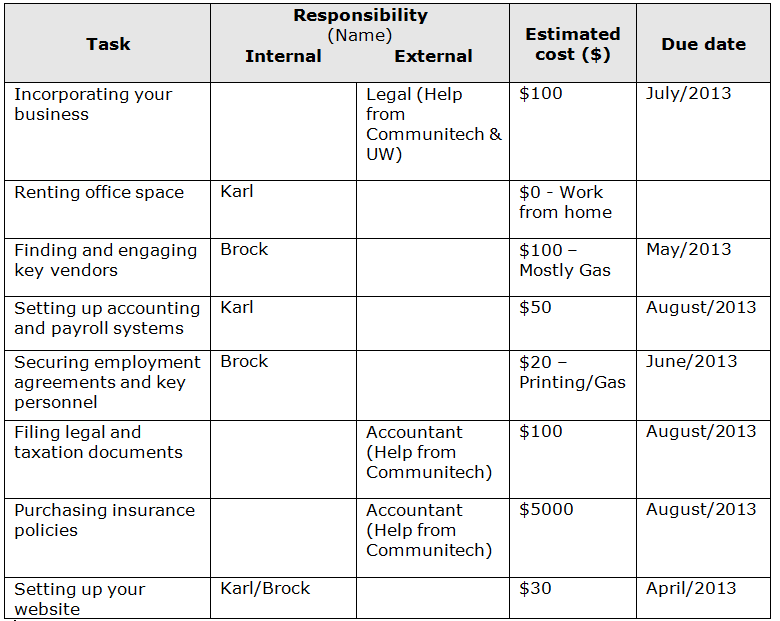
\includegraphics[width=150mm]{images/TaskList.png}
\caption{Task Breakdown}
\label{tasks}
\end{figure}

\subsection{Growth Plan}
The stepping stones described in the Go-to-Market Strategy section of the plan are reiterated in the following financing roadmap. The necessary funding required for each step is presented underneath the appropriate stepping stone.

\begin{figure}[ht!]
\centering
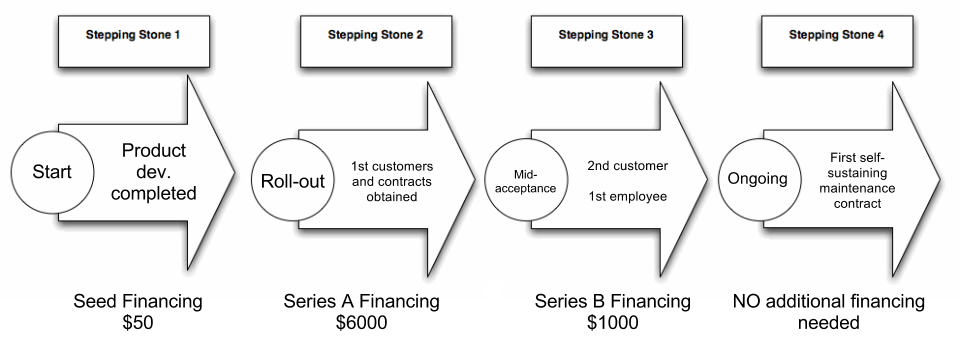
\includegraphics[width=150mm]{images/MSCI454-FinancingRoadmap.png}
\caption{Financing Roadmap}
\label{steppingStones}
\end{figure}
 
Initially only \$150 seed financing will be required. This will cover menial costs associated with working from home and developing {\it Acknowledgements}. This cost does not account for compensating founders during the initial development phase as the co-founders will not be compensated until the first clients have been established.

Series A financing entails purchasing the required server space to host our application for our client to access it before we have started to receive revenue. The rest of the costs associated with this stage of financing are associated with travel to and from client meetings.

Series B financing is again to cover small costs that have to do with client meetings. All necessary expansion costs are covered by the revenue obtained by initial client membership fees.

During the ongoing phase, {\it Acknowledgements} is self-sustaining based on revenue and does not need additional financing.

% \subsection{Pitch Scenarios}
% Ideally, you can provide two sales scenarios based on a high and low case to show the sensitivity and range for your plan.

\subsection{Accounting}
The {\it Acknowledgements} Balance Sheet for the first year is presented in the following table. This Balance Sheet does not account for the development hours worked by the founders, who will not initially be compensated for their work.

\begin{table}[ht]
\caption{The Balance Sheet} % title of Table
\centering % used for centering table
\begin{tabular}{| l | p{1in} | p{1in} | p{1in} |} % centered columns (4 columns)
\hline
{\bf Item of Service} & {\bf Cost per Unit  (\$)} &  {\bf Quantity in First Year } &  {\bf Cost for First Year (\$) } \\
\hline
 &   &   &   \\
{\bf Office (Work from home)} & & & \\
	Computers & 1,500 & 2 & 3,000 \\
	Internet Service & 60 & 12 & 720 \\
	Office Supplies & 300 & 1 & 300 \\
	Printer & 150 & 1 & 150 \\
 &   &   &   \\
{\bf Product} &   &   &   \\
	Web Hosting & 150 & 1 & 150 \\
	Development Hours (unpaid) & 0 & 750 & 0 \\
	Development Hours (paid) & 30 & 1000 & 30,000 \\
  &   &   &   \\
{\bf Client Meetings} &   &   &   \\
	Lunches & 50 &  50 & 2,500\\
	Gas & 50 & 20 & 1,000 \\
  &   &   &   \\
{\bf Legal} &   &   &   \\
	Incorporation & 300 &  1 & 300\\
	Insurance & 5,000 & 1 & 5,000 \\
 &   &  &   \\ 
{\bf Total} &   &   & {\bf 43,120} \\
\hline
\end{tabular}
\label{balanceSheet} % is used to refer this table in the text
\end{table}
\section{Risk Analysis}

{\bf Acknowledgements} is positioned to enter a niche market with currently sparse competition. While this may be true now, with success competition is soon to quickly enter the market. As such 3 critical success factors have been identified to assure that Acknowledgements evolves into a market leader for technical document tracking and approval.

The industry reputation of {\bf Acknowledgements} will be based on a clean and user-friendly interface which allows a user to easily utilize the powerful and secure management and tracking system that corporations will rely on. As such it will be paramount that all releases of the software are thoroughly tested not only for process integrity, but also ease of use. Many applications are known to have started with a simple and clean interface, only to become cluttered and confusing as functionality is added. User testing and closed loop feedback will be important to not only gaining, but sustaining a reputation as the most productive product on the market.

One of the largest weaknesses of web-applications is server failure. Any down-time will have a significant negative impact on the reputation of {\bf Acknowledgements}. Risk of application down-time will be mitigated by using a distributed hosting service, where {\bf Acknowledgements} is hosted by one company, but in various geographic locations. This will result in a much more robust hosting solution that will be resistant to technological failures or ``acts of god''. Another cause of down-time is an application update which causes a critical failure. In order to mitigate this potential issue, all updates will be performed with a full live backup of the previous software release ready to be reinstated. As such, if there is an issue with the update, the old version will be reinstated within minutes of the error being detected. Update cycles will also make use of weekends to assure that updates are performed during periods of minimal application use.

Due to the nature of liability in the construction industry, {\bf Acknowledgements'} approval system will only truly be tested in the event of a catastrophe. It will be during these times that it is critical that {\bf Acknowledgements} is able to produce a full report of exactly which documents were approved by who and in what sequence to assure that liability can be assigned clearly and accurately. Failing to provide an accurate report of the approval process will significantly undermine the reputation of {\bf Acknowledgements} and could immediately put the company's reputation in disrepute. Integrity testing will be constantly undertaken with projects selected at random. This will assure that any issues are discovered before they come to light.

% \begin{center} \begin{tabular}{| p{1in} | p{1.75in} | p{3in} | }
\begin{center} \begin{tabular}{| p{2in} | p{4in} | }
    \hline
    % {\bf Type of Risk} & {\bf Risk} & {\bf Mitigating Strategy} \\ \hline
    {\bf Risk} & {\bf Mitigating Strategy} \\ \hline
	
    % {Product} & 
	{Product does not have required functionality} & 
	{This possibility has been deemed very unlikely due to the foreseen simplicity of implementation. If the product is not ready according to development schedule, more time will be taken rather than rushing an incomplete product to market.} \\ \hline
	
    % {Market Adoption} & 
	{\raggedright Client not interested in trying {\bf Acknowledgements}} & 
	{Contacts within existing companies will be leveraged to assure the product meets client requirements before release.} \\ \hline
	
    % {Market Size Risk} & 
	{The existing market is smaller than anticipated} & 
	{Thorough market research has proven an existing market for {\bf Acknowledgements}. Acknowledgements also has a potential market in the manufacturing industry where technical drawings also require constant revisions and approval.} \\ \hline
	
    % {Financing Risk} & 
	{Insufficient funds to develop or sustain {\bf Acknowledgements}} & 
	{Development plans minimize development cost to avoid this. Alternative financing will be sought from financial institutions should this occur once clients have been established.} \\ \hline

    % {Execution Risk} & 
	{{\bf Acknowledgements} is the first corporation for this management team.} & 
	{The Acknowledgement executive team have worked together for years on various initiatives. They will supplement their knowledge with help from industry advisors.} \\ \hline
\end{tabular} \end{center}

\end{document}
